\documentclass[10pt,compress]{beamer}
\usepackage{xspace}
\usepackage{tikz,pgfplots}
\usepackage{comment}
\usepackage[vlined,linesnumbered]{algorithm2e}

\definecolor{darkred}{HTML}{A60000}
\definecolor{lightblue}{HTML}{4B8EC8}
\definecolor{darkgreen}{HTML}{009000}
\definecolor{lightbrown}{HTML}{AB6402}
\definecolor{yellow9}{HTML}{EC811B}
\definecolor{blackish}{HTML}{23373B}

%% https://github.com/matze/mtheme.git
\usetheme{m}

\usepackage{fontspec}
\usepackage{newunicodechar}
\newcommand{\DeclareUnicodeCharacter}[2]{%
  \begingroup\lccode`|=\string"#1\relax
  \lowercase{\endgroup\newunicodechar{|}}{#2}%
}
  
\usepackage[utf8]{inputenc}  % UTF-8 input encoding

% UNICODE conversion
% greek letters

% Α α Β β Γ γ Δ δ Ε ε Ζ ζ Η η Θ θ Ι ι Κ κ Λ λ Μ μ Ν ν Ξ ξ Ο ο Π π Ρ ρ Σ σ Τ τ Υ υ Φ φ Χ χ Ψ ψ Ω ω

\DeclareUnicodeCharacter{03B1}{\ensuremath{\alpha}}
\DeclareUnicodeCharacter{03B2}{\ensuremath{\beta}}
\DeclareUnicodeCharacter{03B3}{\ensuremath{\gamma}}
\DeclareUnicodeCharacter{0393}{\ensuremath{\Gamma}}
\DeclareUnicodeCharacter{03B4}{\ensuremath{\delta}}
\DeclareUnicodeCharacter{0394}{\ensuremath{\Delta}}
\DeclareUnicodeCharacter{03B5}{\ensuremath{\varepsilon}}
\DeclareUnicodeCharacter{03B6}{\ensuremath{\zeta}}
\DeclareUnicodeCharacter{03B7}{\ensuremath{\eta}}
\DeclareUnicodeCharacter{03B8}{\ensuremath{\vartheta}}
\DeclareUnicodeCharacter{0398}{\ensuremath{\Theta}}
\DeclareUnicodeCharacter{03BA}{\ensuremath{\kappa}}
\DeclareUnicodeCharacter{03BB}{\ensuremath{\lambda}}
\DeclareUnicodeCharacter{039B}{\ensuremath{\Lambda}}
\DeclareUnicodeCharacter{00B5}{\ensuremath{\mu}}      % micron sign
\DeclareUnicodeCharacter{03BC}{\ensuremath{\mu}}
\DeclareUnicodeCharacter{03BD}{\ensuremath{\nu}}
\DeclareUnicodeCharacter{03BE}{\ensuremath{\xi}}
\DeclareUnicodeCharacter{039E}{\ensuremath{\Xi}}
\DeclareUnicodeCharacter{03B9}{\ensuremath{\iota}}
\DeclareUnicodeCharacter{03C0}{\ensuremath{\pi}}
\DeclareUnicodeCharacter{03A0}{\ensuremath{\Pi}}
\DeclareUnicodeCharacter{03C1}{\ensuremath{\rho}}
\DeclareUnicodeCharacter{03C3}{\ensuremath{\sigma}}
\DeclareUnicodeCharacter{03A3}{\ensuremath{\Sigma}}
\DeclareUnicodeCharacter{03C4}{\ensuremath{\tau}}
\DeclareUnicodeCharacter{03C6}{\ensuremath{\varphi}}
\DeclareUnicodeCharacter{03A6}{\ensuremath{\Phi}}
\DeclareUnicodeCharacter{03C7}{\ensuremath{\chi}}
\DeclareUnicodeCharacter{03C8}{\ensuremath{\psi}}
\DeclareUnicodeCharacter{03A8}{\ensuremath{\Psi}}
\DeclareUnicodeCharacter{03C9}{\ensuremath{\omega}}
\DeclareUnicodeCharacter{03A9}{\ensuremath{\Omega}}
\DeclareUnicodeCharacter{03C5}{\ensuremath{\upsilon}}
\DeclareUnicodeCharacter{03A5}{\ensuremath{\Upsilon}}

% some modified characters
\DeclareUnicodeCharacter{1FF6}{\ensuremath{\tilde{\omega}}}

% useful math symbols
\DeclareUnicodeCharacter{221A}{\sqrt}
\DeclareUnicodeCharacter{2264}{\leq}
\DeclareUnicodeCharacter{2265}{\geq}
\DeclareUnicodeCharacter{221E}{\infty}
\DeclareUnicodeCharacter{2211}{\sum}
\DeclareUnicodeCharacter{2208}{\in}
\DeclareUnicodeCharacter{2209}{\notin}
\DeclareUnicodeCharacter{2202}{\partial}
\DeclareUnicodeCharacter{222B}{\int}
\DeclareUnicodeCharacter{2148}{\id}  
\DeclareUnicodeCharacter{2248}{\approx}  
\DeclareUnicodeCharacter{2260}{\neq}  
\DeclareUnicodeCharacter{00B1}{\pm}  
\DeclareUnicodeCharacter{2A02}{\otimes}
\DeclareUnicodeCharacter{2A01}{\oplus}
\DeclareUnicodeCharacter{00BD}{\nicefrac{1}{2}}
\DeclareUnicodeCharacter{00D7}{\times}
\DeclareUnicodeCharacter{00B7}{\cdot}
\DeclareUnicodeCharacter{22C5}{\cdot}
\DeclareUnicodeCharacter{2190}{\gets}

% the prime
\DeclareUnicodeCharacter{2032}{\ensuremath{'}}

% daggers don't need to be preceded by a '^' anymore
\DeclareUnicodeCharacter{2020}{^{\dagger}}
\DeclareUnicodeCharacter{1D40}{^{\textnormal{\tiny{T}}}}
\DeclareUnicodeCharacter{00B2}{^{2}}
\DeclareUnicodeCharacter{00B3}{^{3}}
\DeclareUnicodeCharacter{00BD}{\ensuremath{\frac{1}{2}}\xspace}

% bracket heaven
\DeclareUnicodeCharacter{2329}{\langle}
\DeclareUnicodeCharacter{232A}{\rangle}
\DeclareUnicodeCharacter{27E8}{\langle}
\DeclareUnicodeCharacter{27E9}{\rangle}
\DeclareUnicodeCharacter{2016}{\|}

% fun with arrows
\DeclareUnicodeCharacter{2192}{\to}
\DeclareUnicodeCharacter{21D2}{\implies}
\DeclareUnicodeCharacter{21A6}{\mapsto}
\DeclareUnicodeCharacter{21A9}{\hookleftarrow}

% specialized math letters
\DeclareUnicodeCharacter{2113}{\ell}
\DeclareUnicodeCharacter{210B}{\h}
\DeclareUnicodeCharacter{2115}{\bN}
\DeclareUnicodeCharacter{211D}{\bR}
\DeclareUnicodeCharacter{2102}{\bC}
\DeclareUnicodeCharacter{2119}{\Pr}
\DeclareUnicodeCharacter{2130}{\sE}
\DeclareUnicodeCharacter{2133}{\cM}

% other notation
\DeclareUnicodeCharacter{00B7}{\ensuremath{\cdot}\xspace}
\DeclareUnicodeCharacter{2261}{\ensuremath{\equiv}\xspace}


\usepackage[english]{babel}
\usepackage{booktabs}
\usepackage{numprint}

%Tikz related stuff
\usepackage{tikz}
\usetikzlibrary{fadings}
\tikzstyle{selected} = [fill=blue!30,draw=black,thick,
       preaction={
         fill=black,opacity=.6,
         transform canvas={xshift=0.7mm,yshift=-0.7mm}
       }]
\tikzstyle{round} = [fill=red!30, rounded corners=2pt]


\newcommand{\xor}{\oplus}
\newcommand{\Z}{\mathbb{Z}}
\newcommand{\N}{\mathbb{N}}
\newcommand{\F}{\mathbb{F}}

%setup;online;total time for single-block and lan
\newcommand{\ssl}{\bf 0.002}
\newcommand{\osl}{0.06}
\newcommand{\tsl}{0.06}

%setup;online;total time for single-block and wan
\newcommand{\ssw}{0.14}
\newcommand{\osw}{1.46}
\newcommand{\tsw}{1.61}

%setup;online;total time for multi-block and lan
\newcommand{\sml}{43.33}
\newcommand{\oml}{2.02}
\newcommand{\tml}{45.36}

%setup;online;total time for multi-block and wan
\newcommand{\smw}{138.63}
\newcommand{\omw}{17.12}
\newcommand{\tmw}{155.75}

\newcommand{\simonso}{\bf 0.002}



\title[LowMC]{Ciphers for MPC and FHE}

\author{\textbf{Martin Albrecht}\inst{1} \and  Christian Rechberger\inst{2} \and  Thomas~Schneider\inst{3} \and Tyge Tiessen\inst{2} \and Michael Zohner\inst{3}
}
\institute{
      \inst{1} Royal Holloway, University of London, UK
      \and 
      \inst{2} DTU Compute, Technical University of Denmark, Denmark 
      \and
      \inst{3} TU Darmstadt, Darmstadt, Germany
      }


\date{ICMS, Security of symmetric ciphers in network protocols, Edinburgh}

\begin{document}

\begin{frame}
  \titlepage{}
\end{frame}


\section{Introduction}
\subsection{Motivation}

\begin{frame}{MPC Motivations}
Block ciphers have various applications in MPC
\begin{columns}[T]
\begin{column}{0.23\textwidth}
  \centering
  \vspace{0.2cm}
  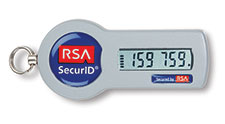
\includegraphics[scale=0.25]{figures/rsatoken.jpg}\\[0.7cm]
  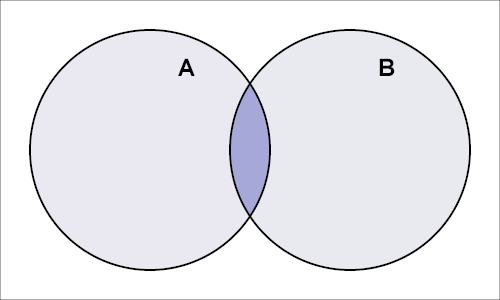
\includegraphics[scale=0.12]{figures/intersection.png}\\[0.3cm]
  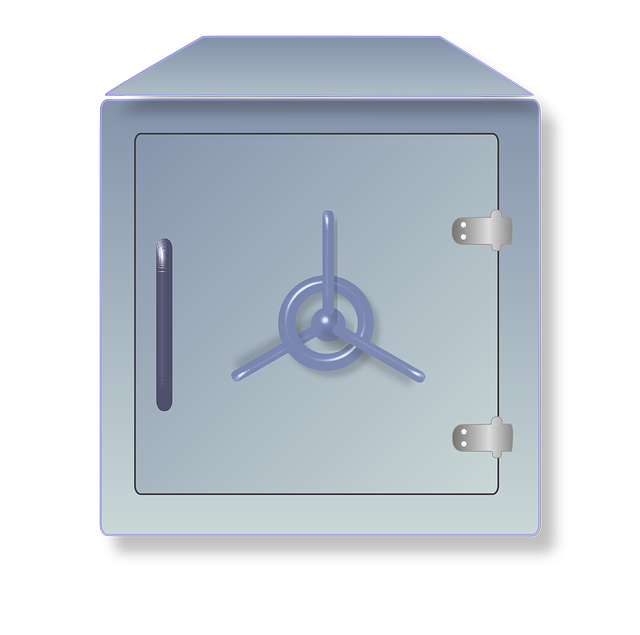
\includegraphics[scale=0.1]{figures/vault.png}
\end{column}
\begin{column}{0.77\textwidth}
  \begin{itemize}
  \item \alert{Server-side one-time passwords}, commercialized by Dyadic Security (server-side derivation of one-time passwords via MPC)
  \item Oblivious Pseudorandom Functions (OPRFs) for \alert{privacy-preserving keyword search}, \alert{private set intersection}, \alert{secure database join}, etc.
  \item \alert{Secure storage}: store symmetrically encrypted intermediate MPC values in untrusted storage
  \end{itemize}
\end{column}
\end{columns}
\end{frame}

\begin{frame}{FHE Motivation}
\begin{columns}
\begin{column}{.4\textwidth}
\begin{tikzpicture}[scale=0.8, every node/.style={scale=0.8}]
  \node[draw, minimum height=1.8cm, minimum width=.7cm, fill=yellow9!50] at (0.5,7.4) (ma) {$m$};
  \node[draw, minimum size=3.6cm, fill=yellow9!50] at (3.5,6.5) (mb) {$\mathrm{HE_{pk}}(m)$};
  \draw[->] (ma) -- (mb);

  \node[draw, minimum height=1.8cm, minimum width=0.7cm, fill=lightblue!50] at (0.5,3) (m1) {$m$};
  \node[draw, fill=yellow9!50] at (0.5,1.5) (k1) {$k$};

  \node[draw, minimum height=0.7cm, minimum width=1.8cm, fill=lightblue!50] at (4.5,2.45) (m2) {$\mathrm{Enc}_k(m)$};
  \node[draw, minimum height=0.7cm, minimum width=1.8cm, fill=yellow9!50] at (4.5,1.5) (k2) {$\mathrm{HE_{pk}}(k)$};
  
  \draw[->] (m1) -- (m2);
  \draw[->] (k1) -- (k2);
\end{tikzpicture}

\end{column}
\begin{column}{.6\textwidth}
FHE schemes typically come with a ciphertext expansion in the order of \alert{1000s} to
\alert{1000000s}. \\[1cm]

\alert{Solution}:\\
\alert{Encrypt message symmetrically}, transfer key homomorphically.\\
Cloud then decrypts homomorphically.
\end{column}
\end{columns}
\end{frame}

\begin{frame}{New computational models require new designs}
\begin{columns}
\begin{column}{0.25\textwidth}
  \centering
  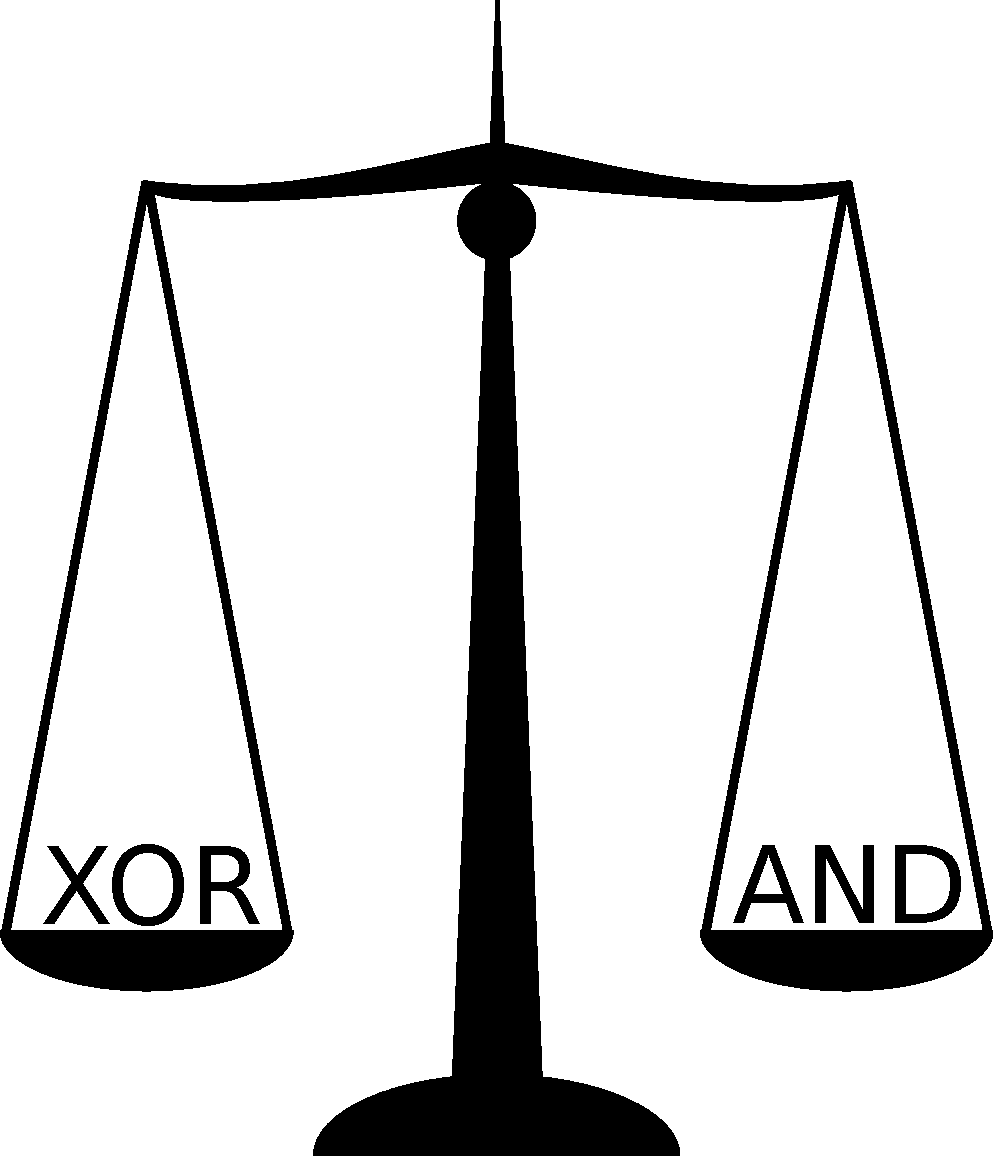
\includegraphics[scale=0.15]{figures/scale.pdf}\\[0.3cm]
  {\huge $\Downarrow$}\\[0.3cm]
  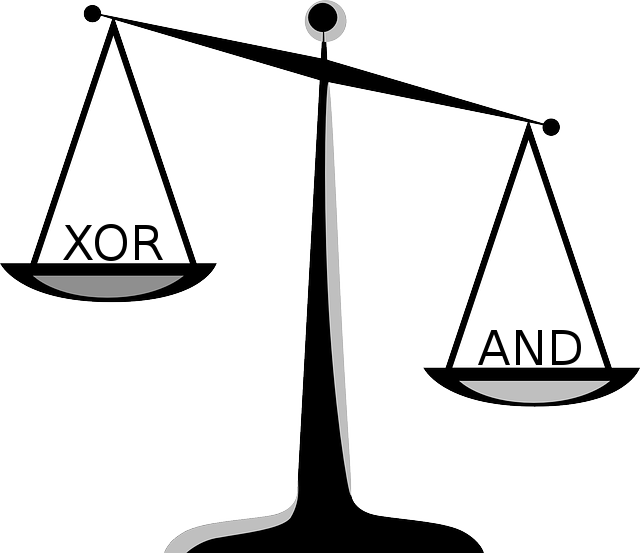
\includegraphics[scale=0.12]{figures/scale.png}
\end{column}
\begin{column}{0.75\textwidth}
\begin{itemize}
\item Since 1970s: balance between linear and non-linear operations because AND gates and XOR gates are roughly the same in most hardware.
\item But cost of XOR gate is (almost) negligible compared to AND gate in MPC or FHE setting
\item Idea: Explore \alert{extreme} trade-offs
\end{itemize}
\begin{alertblock}{Our Guiding Question}
  What would an efficient cipher look like if linear operations were for free?
\end{alertblock}
\end{column}
\end{columns}
\end{frame}

\begin{frame}{Possible metrics for optimisation}
There are three possible metrics to minimise:
\begin{enumerate}
  \item ANDs per bit of encrypted text (\alert{ANDs/bit})
  \item multiplicative depth of the encryption circuit (\alert{ANDdepth})
  \item total number of ANDs per encryption (\alert{ANDs})
\end{enumerate}
\begin{alertblock}{Refined Guiding Question}
  Can we design a cipher that can be optimized with regard to any combination of these
  metrics?
\end{alertblock}
\end{frame}

\begin{frame}{Related work}
Minimisation of multiplicative complexity also relevant in side-channel countermeasures. However, such designs are much less extreme:
\begin{itemize}
  \item Noekeon
  \item Fantomas
  \item Robin 
\end{itemize}
\vspace{0.3cm}

\footnotesize{
Joan Daemen, Micha\"{e}l Peeters, Gilles Van Assche, and Vincent Rijmen.
Nessie proposal: Noekeon. In \textit{First Open NESSIE Workshop}, 2000.\\[0.3cm]

Vincent Grosso, Ga\"{e}tan Leurent, Fran\c{c}ois-Xavier Standaert, and Kerem Varici. LS-designs: Bitslice encryption for efficient masked software implementations. In \textit{Fast Software Encryption (FSE 2014)}, LNCS. Springer.}
\end{frame}


\subsection{Design of the Cipher}

\begin{frame}{Design Strategy}
\begin{alertblock}{Design Ideas}
Minimise ANDs needed for confusion, maximise diffusion.
\end{alertblock}
\begin{itemize}
 \item Use a Substitution-Permutation network (SPN)
 \item Use small S-boxes with low multiplicative complexity
 \item Utilise a partial substitution layer
 \item Maximise diffusion in affine layer
\end{itemize}\end{frame}


\begin{frame}{The LowMC round function and parameters}
\begin{figure}
  \centering
  \begin{tikzpicture}
 [scale=1, every node/.style={scale=1},
  rounded corners, thick,
  sbox/.style={draw,fill=lightblue!50,minimum size=0.7cm},
  affine/.style={draw, fill=lightblue!50, minimum height=0.6cm, minimum width=8.1cm},
  xor/.style = {
    draw, circle, inner sep=0cm, minimum size=0.2cm,
    append after command = {
      [shorten >=\pgflinewidth, shorten <=\pgflinewidth,]
      (\tikzlastnode.north) edge (\tikzlastnode.south)
      (\tikzlastnode.east) edge (\tikzlastnode.west)
    }
  }]
   
  \foreach \x in {1,2,3,4.4,5.4} {
    \draw node[sbox]  at (\x,2) (S) {S};
    \foreach \i in {-1,0,1} \draw (S.south)  ++(0.2*\i,0) -- +(0,-0.35);
    \foreach \i in {-1,0,1} \draw (S.north)  ++(0.2*\i,0) -- +(0,0.35);
  }
  \node at (3.7,2) {$\dots$};
  \foreach \i in {0,...,4} \draw  (6.2+0.2*\i,2.7) -- +(0,-1.4);
  \node at (7.3,2) {$\dots$};
  \foreach \i in {7,...,12} \draw  (6.2+0.2*\i,2.7) -- +(0,-1.4);

  \draw node[affine] at (4.7,1.0) {Affine Layer};
  
  \foreach \i in
      {0,1,2,5,6,7,10,11,12,17,18,19,22,23,24,27,28,29,30,31,34,35,36,37,38,39}
    {
      \draw (0.8+0.2*\i,0.7) -- ++(0,-0.6);	
      \node[xor] at (0.8+0.2*\i,0.4) {};
    }
    
  \draw (9.2,0.4) node (rk) { $k_i$};
  \draw (rk) -- +(-1,0);


%  0.65
%  8.6+0.15=8.75
\end{tikzpicture}

\end{figure}
Size parameters
\begin{itemize}
 \item \alert{block size} $n$ bits
 \item \alert{number of S-boxes} $m$ in substitution layer
\end{itemize}
Security parameters
\begin{itemize}
 \item \alert{key size} $k$
 \item permitted \alert{data complexity} $d$
\end{itemize}
Number of \alert{rounds} $r$ is calculated as a function of the above.
\end{frame}


\begin{frame}{Choice of the S-box}
\begin{alertblock}{S-box Properties}
  \begin{itemize}
  \item maximum differential probability $2^{-2}$
  \item maximum linear probability $2^{-2}$
  \item circuit needs only 3 AND gates and has ANDdepth 1
  \item any combination of output bits has algebraic degree 2
  \end{itemize}
\end{alertblock}
Algebraic Normal Form of S-box:
\begin{align*}
  \color{lightblue} S_0(A,B,C) & \color{lightblue} = A  \oplus \color{yellow9}{BC} \\
  \color{lightblue} S_1(A,B,C) & \color{lightblue} = A  \oplus B \oplus \color{yellow9}{AC}\\
  \color{lightblue} S_2(A,B,C) & \color{lightblue} = A  \oplus B  \oplus C  \oplus \color{yellow9}{AB}
\end{align*}
\end{frame}

\begin{frame}{Maximise diffusion in affine layer}
How do we maximise diffusion in affine layer?
\begin{itemize}
\item \alert{Choose most general affine layer}: multiplication with $n\times n$ matrix over $\F_2$ and addition of constant $\F_2$ vector of length $n$.
\end{itemize}
How do we choose good matrices and vectors?
\begin{itemize}
\item Unfortunately, determining branch number of a binary matrix is hard in practice and theory.
\end{itemize}
We thus
\begin{itemize}
\item \alert{choose random matrices} uniformly from all invertible $n\times n$ matrices over $\F_2$.
\item \alert{choose random constant vectors} uniformly from $\F_2^n$.
\end{itemize}
\alert{Bonus:} This allows novel security arguments.
\end{frame}

\begin{frame}{Key schedule}
Reuse random matrix approach for key schedule:
\begin{itemize}
\item Derive round keys from general key by multiplication with $n\times k$ binary matrix.
 \item Choose matrices uniformly at random from all binary $n\times k$
   matrices of rank $\min(n,k)$.
\end{itemize}
\end{frame}

\begin{frame}{Instantiation of affine layers and round key matrices}
\begin{alertblock}{Problem: How do you accountably instantiate the random matrices and vectors?}
\begin{itemize}
  \item instance of cipher cannot use "random" matrices but must use fixed ones
  \item how choose them in an accountable way ("nothing up the sleeve")?
\end{itemize}
\end{alertblock}
Our solution:
\begin{itemize}
 \item \alert{Use Grain LFSR as self-shrinking generator} to produce random bit string
 \item Then use this string to generate the matrices.
\end{itemize}
\end{frame}

\section{``Free XOR''}

\begin{frame}{Ain't no such thing as free XOR}
  \begin{itemize}
  \item We started our work assuming that XORs are ``essentially free''.
  \item Turns out, ``essentially'' is not ``actually''.
  \item When doing $\approx n^2$ XORs per round this starts to hurt, both in the FHE and the MPC case (in particular in the LAN setting)
  \item We hence use techniques from efficiently linear algebra over $\F_2$ to reduce the cost of matrix-vector products.
  \end{itemize}
\end{frame}


\begin{frame}
\frametitle{Gray Codes}

The Gray code, named after Frank Gray and also known as reflected binary code, is a numbering system where two consecutive values differ in only one digit.
 
\begin{columns}
\column{0.15\textwidth}
\begin{tabular}{c}
0\\
1\\
\end{tabular}

\column{0.30\textwidth}
\begin{tabular}{ccc}
0 & \alert{0} & $\Downarrow$\\
0 & \alert{1} & \\
1 & 1 & \\
1 & 0 & $\Uparrow$\\
\end{tabular}

\column{0.30\textwidth}
\begin{tabular}{ccc}
0 & \alert{0} & \alert{0}\\
0 & \alert{0} & \alert{1}\\
0 & \alert{1} & \alert{1}\\
0 & \alert{1} & \alert{0}\\
1 & 1 & 0\\
1 & 1 & 1\\
1 & 0 & 1\\
1 & 0 & 0\\
\end{tabular}
\end{columns}

\end{frame}

\subsection{Multiplication}

\begin{frame}[fragile]
\frametitle{M4RM}
Consider $w = A \cdot v$ ($A$ is $\in \F_2^{n \times n}$ and $v$ is $\in \F_2^{n}$), where operations on $v$ are expensive.
\vspace{0.2cm}

Divide $A$ into $n/k$ vertical ``stripes'' $A_1 \dots _{n/k}$ of
$k$ columns each. Split $v$ into $n/k$ horizontal ``stripes'' $v_1 \dots v_{n/k}$ of $k$ rows each. We have:

\[
C = A \cdot v = \sum_1^{n/k} A_i \cdot v_i. 
\]
\end{frame}

\begin{frame}[fragile]
\frametitle{M4RM}
\begin{small}
$$A = \left(\begin{array}{rrrr}
1 & 1 & 0 & 1 \\
0 & 0 & 0 & 0 \\
1 & 1 & 1 & 1 \\
0 & 1 & 1 & 1
\end{array}\right), v = \left(\begin{array}{r}
1\\
0\\
0\\
1\end{array}\right),$$
$$A_0 = \left(\begin{array}{rr}
\alert{1} & \alert{1} \\
0 & 0 \\
\alert{1} & \alert{1} \\
0 & 1
\end{array}\right),\ 
A_1 = \left(\begin{array}{rr}
0 & 1 \\
0 & 0 \\
\alert{1} & \alert{1} \\
\alert{1} & \alert{1}
\end{array}\right), v_0 = \left(\begin{array}{rrrr}
1 \\
0
\end{array}\right), v_1 = \left(\begin{array}{rrrr}
0 \\
1
\end{array}\right)
$$
$$
A_0 \cdot v_0 = \left(\begin{array}{rrrr}
\alert{1}\\
0\\
\alert{1} \\
0
\end{array}\right),\ A_1 \cdot v_1 = \left(\begin{array}{rrrr}
1\\
0 \\
\alert{1}\\
\alert{1}
\end{array}\right)$$
\end{small}
\end{frame}

\begin{frame}[fragile]
\frametitle{M4RM: Algorithm $O(n^2/\log n)$}

\begin{algorithm}[H]
\Begin{
$w \longleftarrow $ all zero vector of length $n$\;
$k \longleftarrow \lfloor \log n \rfloor$\;
\For{$0 \le i < (n/k)$}{ 
  {\tcp{create table of $2^k-1$ linear combinations}}
  $T \leftarrow$ \textsc{MakeTable}($v, i\times k, 0, k$)\;
  \For{$0 \le j < n$}{
    {\tcp{\bf read index for table $T$} }
    $id \longleftarrow$ \textsc{ReadBits}($A, j, i \times k, k$)\;
    add row $id$ from $T$ to row $j$ of $w$\;
  }
}
\Return{w}\;
}
\caption{\textsc{M4RM}}
\label{alg:m4rm}
\end{algorithm}

\end{frame}


\section{Security Analysis}

\begin{frame}{To determine round number cryptanalysis necessary}
\begin{alertblock}{Two factors determine the number of rounds}
  \begin{enumerate}
    \item Maximal length of a distinguisher
    \item Number of rounds that can be peeled off
  \end{enumerate}
\end{alertblock}
We investigated the following distinguishers:
\begin{itemize}
  \item Statistical distinguishers: linear and differential characteristics
  \item Low-degree attacks
  \item Combined attacks, special case: Boomerang attacks
\end{itemize}
\end{frame}


\subsection{Differential}

\begin{frame}{Resistance Against Differential attacks}
Standard method to determine probability of best differential characteristic:
\begin{enumerate}
  \item Determine minimal number of active S-boxes.
  \item Combine with maximal differential probability of S-box to determine
        lower bound on best possible characteristic.
\end{enumerate}
To determine the minimal number of active S-boxes the branch number would be helpful.
\begin{alertblock}{Problem}
We do not know the branch number of the randomly chosen matrix.
\end{alertblock}
\end{frame}

\begin{frame}{Bounding differential characteristics}
\begin{columns}
\begin{column}{0.72\textwidth}
\begin{alertblock}{Idea}
  Calculate for each possible good differential characteristic probability that it is realised in instantiation of LowMC\@. Sum all these probabilities to get upper bound for probability that at least one is realised.
\end{alertblock}
Let $C$ be the set of possible good characteristics.
\end{column}
\begin{column}{0.28\textwidth}
  {
  \centering
  \begin{tikzpicture}
  [scale=0.6, every node/.style={scale=0.6},
   rounded corners, thick,
   sbox/.style={draw,fill=lightblue!50,minimum size=0.7cm},
   affine/.style={draw, lightblue!50, minimum height=0.6cm, minimum width=4.8cm},
   active/.style ={fill=yellow9!50}]
   
   %Draw four Sbox/affine layers
   \foreach \y in {2,...,4} {
    \foreach \x in {1,2,3,4} {
      \draw node[sbox]  at (\x,2*\y+0.35) (S\x_\y) {S};
      \foreach \i in {-1,0,1} \draw (S\x_\y.north)  ++(0.2*\i,0) -- +(0,0.35);
      \foreach \i in {-1,0,1} \draw (S\x_\y.south)  ++(0.2*\i,0) -- +(0,-0.35);
      \foreach \i in {-2,-1,0,1} \draw (5,2*\y+0.35)   ++(0.2*\i,0.7) -- +(0,-1.4);
      \draw node[affine] at (3,1.0+2*\y+0.35) {A};
    } 
  }
  %Draw first Sbox layer
  \foreach \y in {2,3,4,5} {
    \foreach \x in {1,2,3,4} {
      \draw node[sbox]  at (\x,2*\y+0.35) (S\x_\y) {S};
      \foreach \i in {-1,0,1} \draw (S\x_\y.south)  ++(0.2*\i,0) -- +(0,-0.35);
      \foreach \i in {-1,0,1} \draw (S\x_\y.north)  ++(0.2*\i,0) -- +(0,0.35);
      \foreach \i in {-2,-1,0,1} \draw (5,2*\y+0.35)   ++(0.2*\i,0.7) -- +(0,-1.4);
    } 
  }
  %Redraw active nodes  
  \draw node[sbox,active] at (S2_5) {S};
  \draw node[sbox,active] at (S1_4) {S};
  \draw node[sbox,active] at (S2_4) {S};
  \draw node[sbox,active] at (S4_4) {S};
  \draw node[sbox,active] at (S3_3) {S};
  \draw node[sbox,active] at (S1_2) {S};
  \draw node[sbox,active] at (S4_2) {S};
  % \draw node[sbox,active] at (S2_1) {S};
  % \draw node[sbox,active] at (S4_1) {S};
\end{tikzpicture}
  }
\end{column}
\end{columns}
\[\sum\limits_{c\in C} \Pr(c\text{ exists in cipher}) \geq \Pr(\text{good characteristic exists})\]
\end{frame}

\begin{frame}
  \frametitle{Bounding Differential Characteristics (Details)}

  \begin{description}
  \item[m] number of S-boxes per layer
  \item[l] bit-length of the identity part of layer
  \item[n] $=3m+l$
  \end{description}

  Let $V(i)$ be the number of $n$-bit vectors encoding a difference activating $i$ S-boxes. 

  \begin{itemize}
  \item We choose $i$ out of the $m$ S-boxes, 
  \item for each active S-box there are 7 possible non-zero input differences and
  \item the bits of the identity part can be chosen freely. So
  \end{itemize}

\[V(i) = \binom{m}{i} \cdot 7^i \cdot 2^l.\]
\end{frame}

\begin{frame}
  \frametitle{Bounding Differential Characteristics (Details)}

  \begin{itemize}
  \item  Let $(α_0, α_1)$ be input/output difference pair for one round.
  \item Let $a_0$ be the number of S-boxes activated by $α_0$. 
  \item An active S-box maps its non-zero input difference to four possible output differences each with probability $\frac{1}{4}$. 
  \item A random binary $n\times n$ matrix maps a given non-zero $n$-bit vector with probability $\frac{1}{2^n-1}$ to another given non-zero output vector.
  \end{itemize}

The probability that the one-round characteristic $(α_0,α_1)$ has a probability larger than 0 is
\[\frac{4^{a_0}}{2^n-1}.\]
\end{frame}

\begin{frame}
  \frametitle{Bounding Differential Characteristics (Details)}

  \begin{itemize}
  \item Let $A = (α_0, α_1, \dots, α_r)$ be a characteristic over $r$ rounds.
  \item Let $(a_0, a_1,\dots, a_{r-1})$ be the numbers of S-boxes activated by $α_0$, $α_1$,$\dots$, and $α_{r-1}$. 
  \end{itemize}

Calculate the probability that $A$ has a probability larger than 0 in a random instantiation of LowMC as
\[\frac{4^{a_0}}{2^n-1}\cdot\frac{4^{a_1}}{2^n-1}\dots\frac{4^{a_{r-1}}}{2^n-1}
    = \frac{4^{a_0+a_1+\cdots + a_{r-1}}}{{(2^n-1)}^r}.\]

\end{frame}

\begin{frame}
  \frametitle{Bounding Differential Characteristics (Details)}

  Summing over all possible $r$-round characteristics that activate at most $d$ S-boxes, calculate an upper bound for the probability that there exists an $r$-round characteristic with $d$ or fewer active S-boxes as
  \[	\sum\limits_{\substack{0\leq a_0,a_1,\dots,a_{r-1}\leq m \\ a_0+a_1+\cdots+a_{r-1}\leq d}}
	V(a_0)\cdot V(a_1)\cdots V(a_{r-1})\cdot (2^n-1)
	\cdot \frac{4^{a_0+a_1+\cdots+a_{r-1}}}{{(2^n-1)}^{r}}
      \]
where the factor $(2^n-1)$ is the number of choices for the last difference $α_r$ that can take any non-zero value.
\end{frame}

\begin{frame}
  \frametitle{Bounding Differential Characteristics (Details)}
  \begin{itemize}
  \item   Each active S-box reduces the probability of a characteristic by a factor of $2^{-2}$. 
  \item From this, calculate the number of rounds after which no good differentials are present except for a negligible probability. 
  \item We consider as good differential characteristics those with a probability higher than $2^{-d}$, where $d$ is the allowed data complexity in the respective parameter set. 
  \item We call a negligible probability a probability lower than $2^{-100}$. 
  \item Note that this probability only comes into play once when fixing an instantiation of LowMC.
  \end{itemize}
\end{frame}

\subsection{Higher-order attacks}

\begin{frame}{Higher Order Attacks}

  \alert{Question:} What is the minimal number of rounds needed to reach a given algebraic degree?

  \begin{lemma}
    If algebraic degree is $d_r$ after $r$ rounds, max.\ degree in round $r+1$ is
    \[\min\left({\color{yellow9}2d_r}, {\color{darkred}m+d_r}, {\color{lightblue}\frac{n}{2}+\frac{d_r}{2}} \right).\]
\end{lemma}
\begin{itemize}
 \item The first bound is trivial.
 \item The second bound is new.
 \item Third bound was proven by Boura, Canteaut, and De Cannière~\cite{DBLP:conf/fse/BouraCC11}
\end{itemize}
\end{frame}


\begin{frame}{Degree Growth}
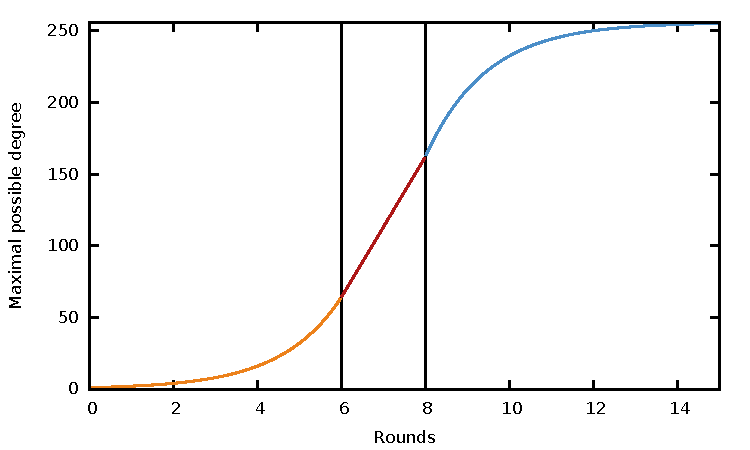
\includegraphics[scale=0.85]{figures/degree.pdf}
\end{frame}

\begin{frame}{Formula to calculate number of rounds}
\begin{alertblock}{Round formula}
\[
 \color{lightblue} r \ge \max(r_{\text{stat}}, r_{\text{deg}}, r_{\text{cmbnd}}) + r_{\text{outer}}
\]
\end{alertblock}
\begin{itemize}
  \item[] {\color{lightblue}$r_{\text{stat}}$}:\qquad  bound for differential and linear distinguishers
  \item[] {\color{lightblue}$r_{\text{deg}}$}:\qquad   bound for sufficient degree
  \item[] {\color{lightblue}$r_{\text{cmbnd}}$}:\quad bound for combined distinguishers
  \item[] {\color{lightblue}$r_{\text{outer}}$}: \quad bound for rounds that can be peeled off
\end{itemize}

For {\color{lightblue}$r_{\text{outer}}$}, we use the ad-hoc formular
\[\color{lightblue}r_{\text{outer}} = r_{\text{stat}}.\]
We thank Dmitry Khovratovich for pointing out that combined attacks can be more effective than others.
\end{frame}

\section{Parameter Sets}

\begin{frame}{Parameters}
 \begin{tabular}{ccccccc}
  \toprule
  S-boxes & blocksize & data & $r_{\text{stat}}$ & $r_{\text{bmrg}}$ &
  $r_{\text{deg}}$ & total rounds \\
  \midrule
  49      &  256       &  $2^{64}$     &  5   &   6   &  6 & 11 \\
  63      &  256       &  $2^{128}$    &  5   &   6   &  7 & 12 \\
  \bottomrule \\
 \end{tabular}
\begin{itemize}
 \item But LowMC is \alert{not limited} to this parameter set
 \item Dependent on optimization metric, size parameters and security
       parameters other parameter sets can be calculated
 \item As \alert{little as 9 rounds} possible for data security of 128~bits
\end{itemize}
\end{frame}

\begin{frame}
  \frametitle{Improved Interpolation Attacks}

  \begin{tabular*}{1.0\linewidth}{rrrrrr}
    \toprule
    Instance & Rounds & Instances\footnote{Over randomness of matrix creation.} & Data     & Time     & Memory   \\
    \midrule
    LowMC-80 & 9/11   & 1/1       & $2^{35}$ &  $2^{38}$ & $2^{35}$\\
             & 10/11  & 1/1       & $2^{39}$ &  $2^{57}$ & $2^{39}$\\
             & 11/11  & $2^{-38}$  & $2^{39}$ &  $2^{57}$ & $2^{39}$\\
    \midrule
    LowMC-128 & 11/12 & 1         & $2^{70}$ &  $2^{86}$ & $2^{70}$\\
              & 12/12 & $2^{-122}$ & $2^{70}$ &  $2^{86}$ & $2^{70}$\\
              & 12/12 & 1         & $2^{73}$ & $2^{118}$ & $2^{80}$\\
    \bottomrule
  \end{tabular*}

  \begin{thebibliography}{FooBar}
  \bibitem[DLMW15]{EPRINT:DLMW15}
    Itai Dinur, Yunwen Liu, Willi Meier, and Qingju Wang
    \newblock Optimized Interpolation Attacks on LowMC
    \newblock Cryptology ePrint Archive, Report 2015/418. 2015
  \end{thebibliography}
\end{frame}

\begin{frame}{Parameter space for AES-like security}
\begin{figure}
\centering
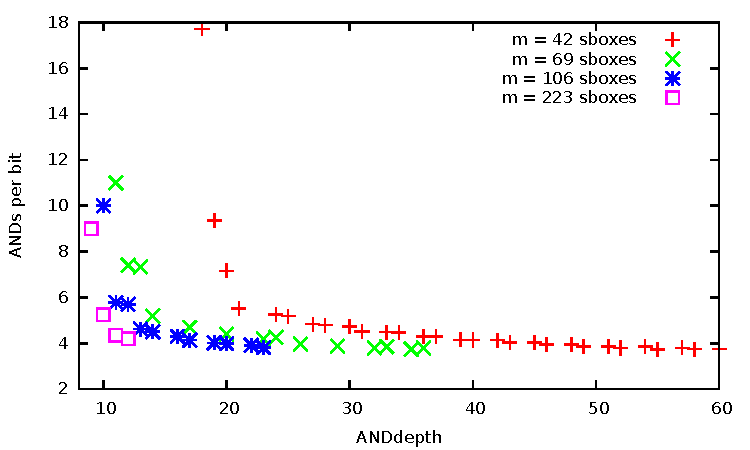
\includegraphics[scale=0.8]{figures/designspace.pdf}
\end{figure}
\end{frame}


\begin{frame}{Comparison with most competitive other ciphers}
\centering
\large{AES-like security}
\scriptsize
\begin{table}
\begin{tabular}{cccccc}
\toprule
Cipher & Key size & Block size & Data sec. & ANDdepth & ANDs/bit \\
\midrule
AES-128 & 128 & 128 & 128 & 40 (60) & 43 (40) \\
%AES-192 & 192 & 128 & 128 & 48 (72) & 51 (48) \\
%AES-256 & 256 & 128 & 128 & 56 (84) & 60 (56) \\
Simon & 128 & 128& 128 & 68 & 34 \\
%Simon & 192 & 128& 128 & 69 & 35 \\
%Simon & 256 & 128& 128 & 72 & 36 \\
Noekeon & 128 & 128& 128 & 32 & 16 \\
Robin & 128 & 128& 128 & 96 & 24 \\
Fantomas & 128 & 128& 128 & 48 & 16.5 \\
%Threefish & 512 & 512 & 512 & 936 (\numprint{4536}) & 306 (36) \\
%Threefish & 512 & \numprint{1024} &1024 &  \numprint{1040} (\numprint{5040}) & 340 (40) \\
\midrule
LowMC & 128 & 256 & 128 & 12 & 8.85 \\
\bottomrule
\end{tabular}
\end{table}
\end{frame}

\begin{frame}{Comparison with most competitive other ciphers}
\centering
\large{Lightweight security}
\scriptsize
\begin{table}
\begin{tabular}{cccccc}
\toprule
Cipher & Key size & Block size & Data sec. & ANDdepth & ANDs/bit \\
\midrule
PrintCipher-96 & 160 & 96 & 96 & 96 & 96 \\
PrintCipher-48 & 80 & 48 & 48 & 48 & 48 \\
Present & 80 or 128 & 64& 64&62 (93) & 62 (31) \\
Simon & 96 & 64& 64&42& 21 \\
Simon & 64 & 32 & 32 & 32 & 16 \\
Prince & 128 & 64& 64&24 & 30 \\
KATAN64 & 80 & 64& 64 & 74 & 36 \\
%KATAN48 & 80 & 48 & 48 & 74 & 32 \\
KATAN32 & 80 & 32& 32& 64 & 24 \\
DES& 56 & 64& 56&261 & 284 \\
\midrule
LowMC & 80 & \numprint{256} & 64 & 11 & 6.31 \\
\bottomrule
\end{tabular}
\end{table}
\end{frame}

\section{Benchmark results}

\begin{frame}{Benchmark results for multiple blocks of total size $12.8$ Mbit in GMW}
\centering
\begin{table}
\scriptsize
\centering
\begin{tabular}{ l r r r r r r}
\multicolumn{7}{l}{\emph{Lightweight Security}} \\
\toprule
Cipher &  \multicolumn{2}{c}{Present} & \multicolumn{2}{c}{Simon} & \multicolumn{2}{c}{LowMC} \\
\midrule
Comm. [GB] & \multicolumn{2}{c}{7.4} & \multicolumn{2}{c}{5.0} & \multicolumn{2}{c}{\bf 2.5} \\
\midrule
 & \multicolumn{1}{c}{LAN} & \multicolumn{1}{c}{WAN} & \multicolumn{1}{c}{LAN} & \multicolumn{1}{c}{WAN} & \multicolumn{1}{c}{LAN} & \multicolumn{1}{c}{WAN} \\
%Setup [s]  & 214.17 & 453.89 & 268.93 & 568.35 &  \bf \sml & \bf \smw \\
%Online [s] &   2.71  & 34.35 &   3.29 &  37.06 &  \bf \oml & \bf \omw \\
Total [s]  & 216.88 & 488.24 & 272.22 & 605.41 &  \bf \tml & \bf \tmw \\
\bottomrule
\\[0.5cm]
\multicolumn{7}{l}{\emph{Long-Term Security}} \\
\toprule
Cipher & \multicolumn{2}{c}{AES} & \multicolumn{2}{c}{Simon} & \multicolumn{2}{c}{LowMC} \\
\midrule
Comm. [GB] & \multicolumn{2}{c}{16} & \multicolumn{2}{c}{13} & \multicolumn{2}{c}{\bf 3.5} \\
\midrule
  & \multicolumn{1}{c}{LAN} & \multicolumn{1}{c}{WAN} & \multicolumn{1}{c}{LAN} & \multicolumn{1}{c}{WAN} & \multicolumn{1}{c}{LAN} & \multicolumn{1}{c}{WAN} \\
%Setup [s] & 553.41 & 914.27 & 444.30 & 727.48 & \bf 62.01    & \bf 193.90 \\
%Online [s] &    2.50 &  33.52 &   2.97 &  34.42 &  \bf 2.36 &  \bf 21.11 \\
Total [s] &   555.91 & 947.79 & 447.27 & 761.90 & \bf 64.37    & \bf 215.01 \\
\bottomrule
\end{tabular}
\end{table}
\end{frame}



\begin{frame}{Benchmark results FHE using HELib by Halevi \& Shoup}
\centering
\begin{table}
\scriptsize
\centering
\begin{tabular}{rrc@{\hskip 1em}r@{\hskip 1em}r@{\hskip 1em}r@{\hskip 1em}r@{\hskip 1em}l@{\hskip 1em}l@{\hskip 1em}l}
\toprule
  $d$  & $n$ & ANDdepth & $t_{block}$ & $t_{bit}$ & Cipher & Ref. & Key Sched.\\
\midrule
 128 & 128 & 40 &  1.5s & 0.0119s & AES-128 & \cite{cryptoeprint:2012:099} & excluded\\
 128 & 128 & 40 &   55s & 0.2580s & AES-128 & \cite{cryptoeprint:2014:039} & excluded\\
 128 & 128 & 40 &   22m & 10.313s & AES-128 & \cite{mella-susella:ima2013} & excluded\\
 128 & 128 & 40 &   14m &  6.562s & AES-128 & \cite{mella-susella:ima2013} & excluded\\
 128 & 256 & 12 &  0.8s & 0.0033s & LowMC   & this work & included\\
\midrule
  64 & size & 24 &  3.3s & 0.0520s & PRINCE  & \cite{cryptoeprint:2014:233} & excluded\\
  64 & 256 & 11 & 0.64s & 0.0025s & LowMC   & this work & included\\  
\midrule
\end{tabular}
\end{table}
\end{frame}

\section{Conclusion}

\begin{frame}{Conclusion}
\begin{itemize}
  \item Proposed \alert{flexible block cipher} design of \alert{extremely low}
        number of \alert{ANDs/bit} and \alert{extremely low ANDdepth}
  \item Provided experimental and theoretical cryptanalysis to ensure
        soundness of design
  \item Demonstrate that symmetric design and cryptanalysis can significantly contribute
        to make applications of MPC and FHE more practical
  \item Measured \alert{speed-up} factors between 2 and 25
\end{itemize}
\end{frame}

\begin{frame}{Open problems}
  \begin{itemize}
  \item Can the cost of LowMC in the traditional setting be reduced by using a sparser affine layer without reducing security claims?
  \item Improve implementations of LowMC in MPC and FHE settings
  \item What designs can minimize the multiplicative complexity over larger fields than $\F_2$?
  \item Further refinement of round number formula, explicitly include key size
  \item Further cryptanalysis needed
\end{itemize}
\end{frame}

\begin{frame}{Thank you}
  \centering
  \alert{\Large Questions?} \\
  \vfill
  \begin{description}
  \item[paper] {\small\url{http://thomaschneider.de/papers/ARSTZ15.pdf}}
  \item[fhe impl.] {\small\url{https://bitbucket.org/malb/lowmc-helib}}
  \item[mpc impl.] {\small\url{https://github.com/encryptogroup/aby}}
  \end{description}
\end{frame}

% All of the following is optional and typically not needed. 
\appendix
\section<presentation>*{\appendixname}
\subsection<presentation>*{For Further Reading}

\begin{frame}
  \frametitle<presentation>{References}
{\tiny
  \bibliographystyle{alpha}
  \bibliography{local}
}
\end{frame}

\end{document}


%%% Local Variables:
%%% mode: latex
%%% TeX-master: t
%%% End:
